\section[پروژه اول: خوشه‌بندی طیفی \lr{(Spectral Clustering)}]{\faProjectDiagram\ \ پروژه اول: خوشه‌بندی کاربران در شبکه‌های اجتماعی با Spectral Clustering}

\begin{stepbox}

\field{۱. هدف و معرفی مسئله}{
هدف از این پروژه، یافتن اجتماع‌ها \lr{(Communities)} و گروه‌بندی رئوس یک گراف همبند است؛ به طوری که رئوس درون یک خوشه بیشترین ارتباط (یال) را با یکدیگر و کمترین ارتباط را با خوشه‌های دیگر داشته باشند. در شبکه‌های اجتماعی، این مسئله معادل یافتن گروه‌های دوستی متراکم است. برای حل این مسئله از الگوریتم خوشه‌بندی طیفی \lr{(Spectral Clustering)} استفاده شده است که به جای استفاده از روش‌های سنتی گراف، مسئله را با استفاده از مقادیر ویژه و بردارهای ویژه‌ی ماتریس‌های گراف به یک مسئله‌ی هندسی و جبر خطی تبدیل می‌کند.
}

\field{۲. تشکیل ماتریس‌های گراف و لاپلاسین \lr{(Graph Laplacian)}}{
الگوریتم با دریافت ماتریس مجاورت \lr{(Adjacency Matrix)} گراف ($A$) آغاز می‌شود. در این ماتریس متقارن، وجود یال بین دو راس $i$ و $j$ با مقدار ۱ و عدم وجود آن با صفر نشان داده می‌شود.
در گام بعدی، ماتریس درجه \lr{(Degree Matrix)} با نام $D$ تشکیل می‌گردد که یک ماتریس قطری است و هر درایه روی قطر اصلی آن، برابر با مجموع درایه‌های سطر متناظر در ماتریس $A$ (تعداد یال‌های متصل به آن راس) است.

سپس ماتریس لاپلاسین گراف \lr{(Laplacian Matrix)} به شکل زیر تعریف می‌شود:
\[
L = D - A
\]
ویژگی مهم ماتریس لاپلاسین این است که مجموع درایه‌های هر سطر آن دقیقاً برابر با صفر است. این ویژگی باعث می‌شود که ماتریس $L$ همواره تکین \lr{(Singular)} بوده و حداقل یک مقدار ویژه‌ی صفر داشته باشد. همچنین این ماتریس مثبت نیمه‌معین \lr{(Positive Semi-Definite)} است، یعنی تمامی مقادیر ویژه‌ی آن نامنفی هستند ($\lambda_i \ge 0$).
}
\newpage
\field{۳. استخراج طیف گراف و بردار فیدلر \lr{(Fiedler Vector)}}{
پس از تشکیل ماتریس لاپلاسین، معادله‌ی مقادیر ویژه ($Lx = \lambda x$) حل شده و مقادیر ویژه به صورت صعودی مرتب می‌شوند. 
همان‌طور که اشاره شد، کوچک‌ترین مقدار ویژه همواره $\lambda_1 = 0$ است. دومین مقدار ویژه‌ی کوچک ($\lambda_2$) که به آن «همبندی جبری» \lr{(Algebraic Connectivity)} می‌گویند، نقش کلیدی در خوشه‌بندی دارد. بردار ویژه‌ی متناظر با این مقدار ویژه، \textbf{بردار فیدلر \lr{(Fiedler Vector)}} نامیده می‌شود.

با بررسی علامت درایه‌های بردار فیدلر، می‌توان گراف را به دو بخش بهینه (برش کمینه یا \lr{Min-Cut}) تقسیم کرد. رئوسی که درایه‌ی متناظرشان در بردار فیدلر مثبت است در یک خوشه، و رئوسی که درایه‌شان منفی یا صفر است در خوشه‌ی دیگر قرار می‌گیرند. این روش ابتدا روی یک گراف تمرینی ۹ راسی با موفقیت تست شد.

\vspace{0.4cm}
\begin{center}
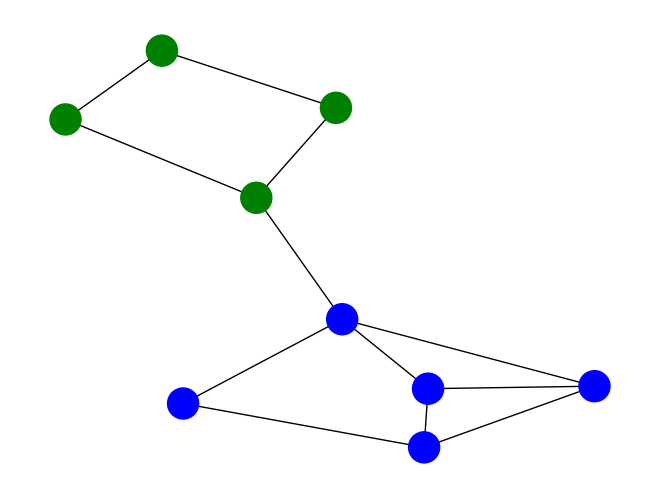
\includegraphics[width=.6\textwidth]{images/graph_dummy_2clusters.png}
\captionof{figure}{خوشه‌بندی گراف ۹ راسی به ۲ خوشه با استفاده از علامت درایه‌های بردار فیدلر}
\label{fig:graph_dummy}
\end{center}
}
\newpage
\field{۴. پیاده‌سازی بر روی گراف اصلی \lr{(Main Graph)}}{
پس از تایید منطق روی گراف تمرینی، الگوریتم روی داده‌های گراف اصلی (شامل ۱۰۰ راس که از فایل متنی استخراج شده بود) اجرا گردید. ماتریس لاپلاسین $100 \times 100$ تشکیل و بردار فیدلر استخراج شد. با اعمال شرط علامت ($x > 0$) روی بردار فیدلر، گراف پیچیده‌ی اصلی به دو اجتماع مجزا و متراکم تقسیم شد.

\vspace{0.4cm}
\begin{center}
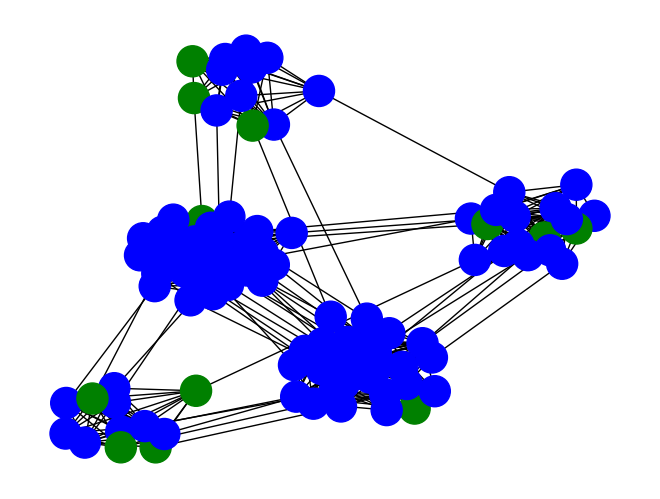
\includegraphics[width=.6\textwidth]{images/graph_main_2clusters.png}
\captionof{figure}{تقسیم‌بندی گراف ۱۰۰ راسی اصلی به ۲ خوشه مجزا با استفاده از بردار فیدلر}
\label{fig:graph_main_2c}
\end{center}
}

\field{۵. بهبود خوشه‌بندی با تعبیه در فضای جدید و الگوریتم \lr{K-Means}}{
برای استخراج تعداد خوشه‌های بیشتر (مثلاً $k=4$)، استفاده‌ی دستی از علامتِ چند بردار ویژه (حالت‌های $+,-$ و ...) دقت بالایی ندارد. رویکرد اصولی در خوشه‌بندی طیفی این است که رئوس گراف در یک فضای هندسی جدید با ابعاد پایین‌تر تعبیه \lr{(Embed)} شوند.

برای خوشه‌بندی به $k$ دسته، $k$ بردار ویژه‌ی اول ماتریس لاپلاسین انتخاب شده و به صورت ستونی کنار هم قرار می‌گیرند تا ماتریس تعبیه \lr{(Embedding Matrix)} با ابعاد $n \times k$ ساخته شود. اکنون هر سطر این ماتریس، مختصات یک راس را در فضای $\mathbb{R}^k$ نشان می‌دهد. در نهایت، با اعمال الگوریتم استاندارد \lr{K-Means} بر روی سطرهای این ماتریس، خوشه‌بندی نهایی و دقیق با هر تعداد دسته‌ی دلخواه استخراج می‌گردد.

\vspace{0.4cm}
\begin{center}
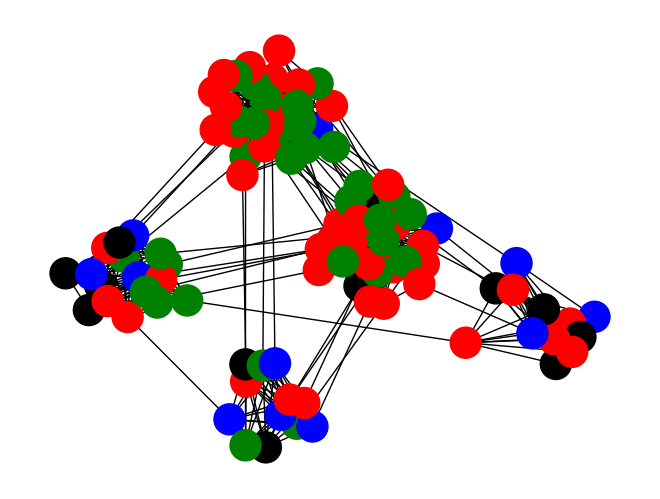
\includegraphics[width=.6\textwidth]{images/graph_main_kmeans.png}
\captionof{figure}{خوشه‌بندی نهایی گراف ۱۰۰ راسی به ۴ خوشه با ترکیب بردارهای ویژه و الگوریتم \lr{K-Means}}
\label{fig:graph_main_kmeans}
\end{center}
}

\field{۶. جمع‌بندی}{
این پروژه نشان داد که چگونه می‌توان یک ساختار گسسته و پیچیده مانند گراف را با استفاده از ماتریس لاپلاسین و طیف آن (مقادیر و بردارهای ویژه) به یک فضای پیوسته‌ی هندسی نگاشت کرد. الگوریتم خوشه‌بندی طیفی، به ویژه زمانی که با \lr{K-Means} ترکیب می‌شود، یکی از قدرتمندترین روش‌ها برای یافتن ساختارهای پنهان و اجتماع‌ها در شبکه‌های پیچیده است که نسبت به الگوریتم‌های سنتی گراف، مقاومت و دقت بسیار بالاتری در برابر نویز و یال‌های تصادفی نشان می‌دهد.
}

\end{stepbox}